\section{Interprete}
\subsection{Diagrammi della classi}
L'interprete è la componente di MaaS che si occupa della conversione da DSL Structure in DSL. Questa decisione è stata presa per poter avere una rappresentazione semplice da manipolare attraverso l'editor e facile da ricondurre nel formato testuale.

La progettazione ha seguito un approccio bottom-up, con la creazione delle componenti per il funzionamento, incluse in un package e inserito un Facade per semplificarne l'uso. I patter usati sono Facade, Singleton e Chain of Responsability.
\subsection{Package DSLInterpreter}
\begin{figure}[H]
  \centering
  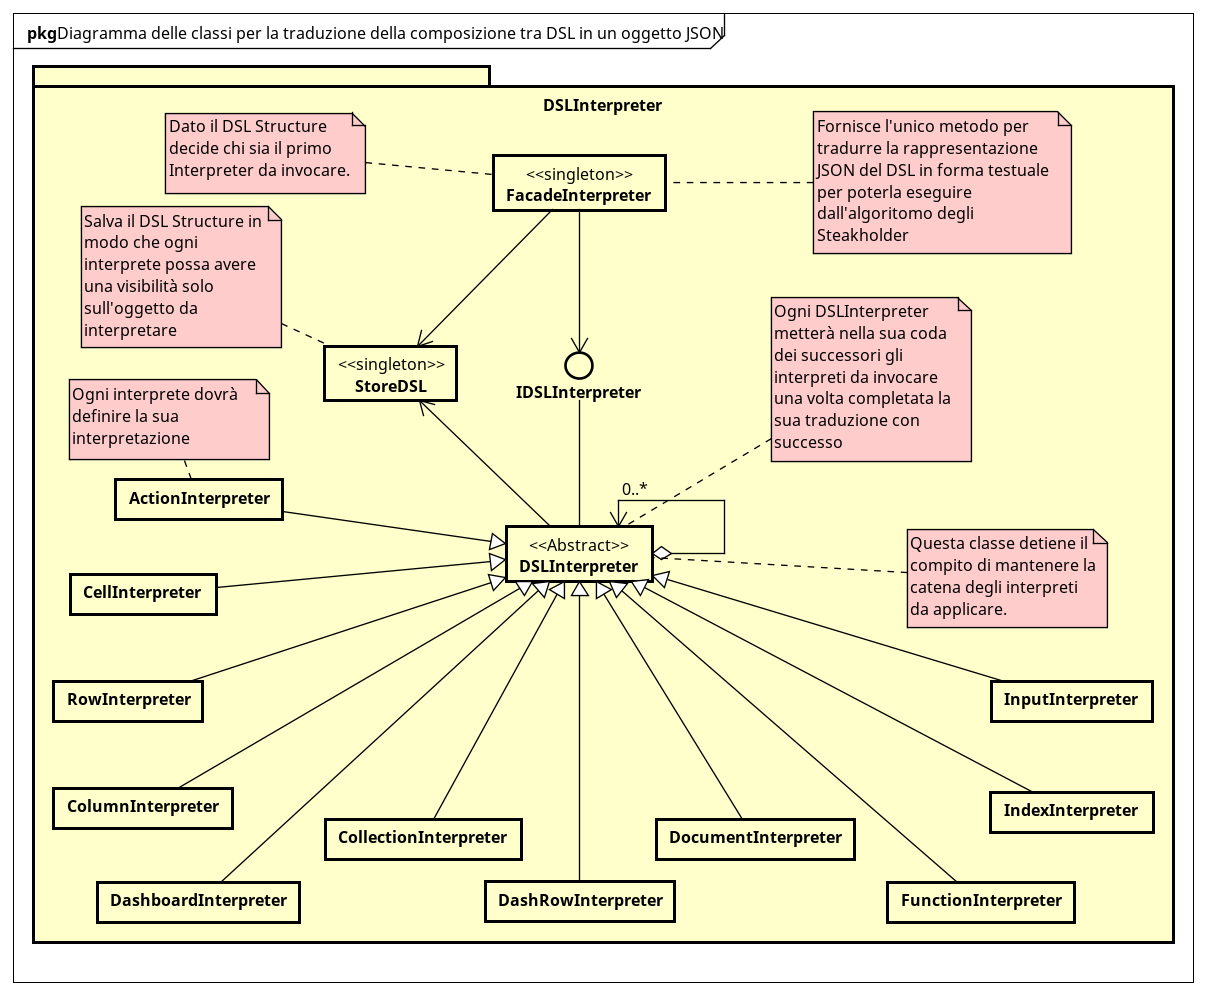
\includegraphics[width=0.9\textwidth]{res/img/Diagram_Interpreter.png}
  \caption{Package DSLInterpreter}
  \label{fig:diagram_model}
\end{figure}
\subsubsection{Descrizione}
In questo package vengono inserite tutte le classi che contribuiscono alla traduzione dal DSL Structure prodotto dall'editor all'equivalente DSL.
La classe DSLInterpreter implementa il Chain of Responsability dove detiene una lista di tutti gli interpreti da invocare man mano che vengono applicate le traduzioni. Il risultato di ogni interprete verrà contatenato e come risultato si otterrà il DSL richiesto.
Il FacadeEditorInterpreter implementa il patter Facade per offrire un interfaccia semplice per attuare la traduzione rendendo nascoste i componenti per applicarla.
\subsubsection{DSLInterpreter::FacadeInterpreter}
\begin{itemize}
\item \textbf{Descrizione} \hfill \\
  Rappresenta l'implementazione del pattern Facade.
\item \textbf{Utilizzo} \hfill \\
  Permette di interfacciarsi al modulo richiedendo eslusivamente la traduzione da DSL Structure a DSL. Questo oltre a semplificare al client la gestione della traduzione, nasconde l'implementazione rendendo il modulo maggiormente mantenibile.
\item \textbf{Relazioni con altre classi} \hfill
  \begin{itemize}
  \item DSLInterpreter::StoreDSL
  \item DSLInterpreter::IDSLInterpreter
  \end{itemize}
\end{itemize}
\subsubsection{DSLInterpreter::StoreDSL}
\begin{itemize}
\item \textbf{Descrizione} \hfill \\
  Mantiene il riferimento dal DSL Structure da tradurre.
\item \textbf{Utilizzo} \hfill \\
  Viene usata dalle implementazioni di \texttt{DSLInterpreter::DSLInterpreter} per ottenere l'oggetto riferito da un attributo della struttura da tradurre. Questi casi si riscontrano nella definizione di un componente del DSL in cui sono innestati altri componenti ( es. DSL Collection con DSL Index e DSL Document ).

  Ciò permette di non violare il Single Responsability Principle, in quanto i vari interpreti conoscono solo la struttura del singolo componente da interpretare e non detengono un possibile accesso dell'intera DSL Structure.
\item \textbf{Relazione con altre classi} \hfill
  \begin{itemize}
  \item DSLInterpreter::DSLFacadeInterpreter
  \item DSLInterpreter::DSLInterpreter
  \end{itemize}
\end{itemize}
\subsubsection{DSLInterpreter::DSLInterpreter}
\begin{itemize}
\item \textbf{Descrizione}
  Implementa il Chain of Responsabiltity mantenendo una lista di tutti gli interpreti da avviare e fornisce i metodo da implementare per i vari interpreti.
\item \textbf{Utilizzo}
  Mantiene struttura dati ed il comportamento comune degli interpreti. In più attraverso il metodo interpret viene definita la sequenza per portare a compito la traduzione di una componente del DSL.
\item \textbf{Relazione con altre classi} \hfill
  \begin{itemize}
  \item DSLInterpreter::FacadeInterpreter
  \item DSLInterpreter::StoreDSL
  \item DSLInterpreter::ActionInterpreter
  \item DSLInterpreter::CellInterpreter
  \item DSLInterpreter::RowInterpreter
  \item DSLInterpreter::ColumnInterpreter
  \item DSLInterpreter::DashboardInterpreter
  \item DSLInterpreter::CollectionInterpreter
  \item DSLInterpreter::DashRowInterpreter
  \item DSLInterpreter::DocumentInterpreter
  \item DSLInterpreter::FunctionInterpreter
  \item DSLInterpreter::IndexInterpreter
  \item DSLInterpreter::InputInterpreter
  \end{itemize}
\end{itemize}

\subsubsection{DSLInterpreter::ActionInterpreter}
\begin{itemize}
\item \textbf{Descrizione}
Implementa la traduzione di un oggetto che rispetti le caratteristiche di un Action Element.
\item \textbf{Utilizzo}
Usato da \texttt{DSLInterpreter::CollectionInterpreter} e \texttt{DSLInterpreter::DocumentInterpreter} per tradurre un Action associato.
\item \textbf{Relazone con altre classi}
\begin{itemize}
\item DSLInterpreter::DSLInterpreter
\item DSLInterpreter::CollectionInterpreter
\item DSLInterpreter::DocumentInterpreter
\end{itemize}
\end{itemize}

\subsubsection{DSLInterpreter::CellInterpreter}
\begin{itemize}
\item \textbf{Descrizione}
Implementa la traduzione di un oggetto che rispetti le caratteristiche di un Cell Element.
\item \textbf{Utilizzo}
Usato da \texttt{DSLInterpreter::FacadeInterpreter} nel caso un Cell Element \'e l'elemento radice del DSL Structure, altrimenti viene creato da \texttt{DSLInterpreter::DashRowInterpreter} quando una Cell compone una riga della Dashboard Element.
\item \textbf{Relazione con altre classi}
\begin{itemize}
\item DSLInterpreter::FacadeInterpreter
\item DSLInterpreter::DSLInterpreter
\item DSLInterpreter::DashRowInterpreter
\end{itemize}
\end{itemize}

\subsubsection{DSLInterpreter::RowInterpreter}
\begin{itemize}
\item \textbf{Descrizione}
Implementa la traduzione di un oggetto che rispetti le caratteristiche di un Row Element.
\item \textbf{Utilizzo}
Usato da \texttt{DSLInterpreter::DocumentInterpreter} per tradurre una Row associata.
\item \textbf{Relazione con altre classi}  
\begin{itemize}
\item DSLInterpreter::DSLInterpreter
\item DSLInterpreter::DocumentInterpreter
\end{itemize}
\end{itemize}

\subsubsection{DSLInterpreter::ColumnInterpreter}
\begin{itemize}
\item \textbf{Descrizione}
Implementa la traduzione di un oggeto che rispetti le caratteristiche di un Column Element.
\item \textbf{Utilizzo}
Usato da \texttt{DSLInterpreter::IndexInterpreter} per tradurre un Column associato.
\item \textbf{Relazione con altre classi}
\begin{itemize}
\item DSLInterpreter::DSLInterpreter
\item DSLInterpreter::IndexInterpreter
\end{itemize}
\end{itemize}

\subsubsection{DSLInterpreter::DashboardInterpreter}
\begin{itemize}
\item \textbf{Descrizione}
Implementa la traduzione di un oggetto che rispetti le caratteristiche di un Dashboard Element.
\item \textbf{Utilizzo}
Usato da \texttt{DSLInterpreter::FacadeInterpreter} nel caso un Dashboard Element \'e l'elemento radice del DSL Structure. 
\item \textbf{Relazione con altre classi}
\begin{itemize}
\item DSLInterpreter::DSLInterpreter
\item DSLInterpreter::FacadeInterpreter
\end{itemize}
\end{itemize}

\subsubsection{DSLInterpreter::CollectonInterpreter}
\begin{itemize}
\item \textbf{Descrizione}
Implemenata la traduzione di un oggetto che rispetti le caratteristiche di un Collection Element.
\item \textbf{Utilizzo}
Usato da \texttt{DSLInterpreter::IndexInterpreter} per tradurre una Index associata.
\item \textbf{Relazione con altre classi}
\begin{itemize}
\item DSLInterpreter::DSLInterpreter
\item DSLInterpreter::IndedInterpreter
\end{itemize}
\end{itemize}

\subsubsection{DSLInterpreter::DashRowInterpreter}
\begin{itemize}
\item \textbf{Descrizione}
Implementa la traduzione di un oggeto che rispetti le caratteristiche di un DashRow Element.
\item \textbf{Utilizzo}
Usato da \texttt{DSLInterpreter::Dashboarda}
\item \textbf{Relazione con altre classi}
\begin{itemize}
\item DSLInterpreter::DSLInterpreter
\item DSLInterpreter::DashboardInterpreter 
\end{itemize}
\end{itemize}
